%!TEX root = ../main_wo_rep.tex
%
% 熱電対
%


\section{熱電対}

\subsection{熱電対とは}

熱電対とは、異なる材料の2本の金属線を接続して1つの回路にしたもののことを 
言います。この熱電対の二つの接点に温度差を与えると、回路に電圧が発生し、電流 
が流れるという現象がおきます。この現象は、1821年にドイツの物理学者トーマス・ 
ゼーベックによって発見され、{\bf ゼーベック効果}と呼ばれています。

\begin{center}
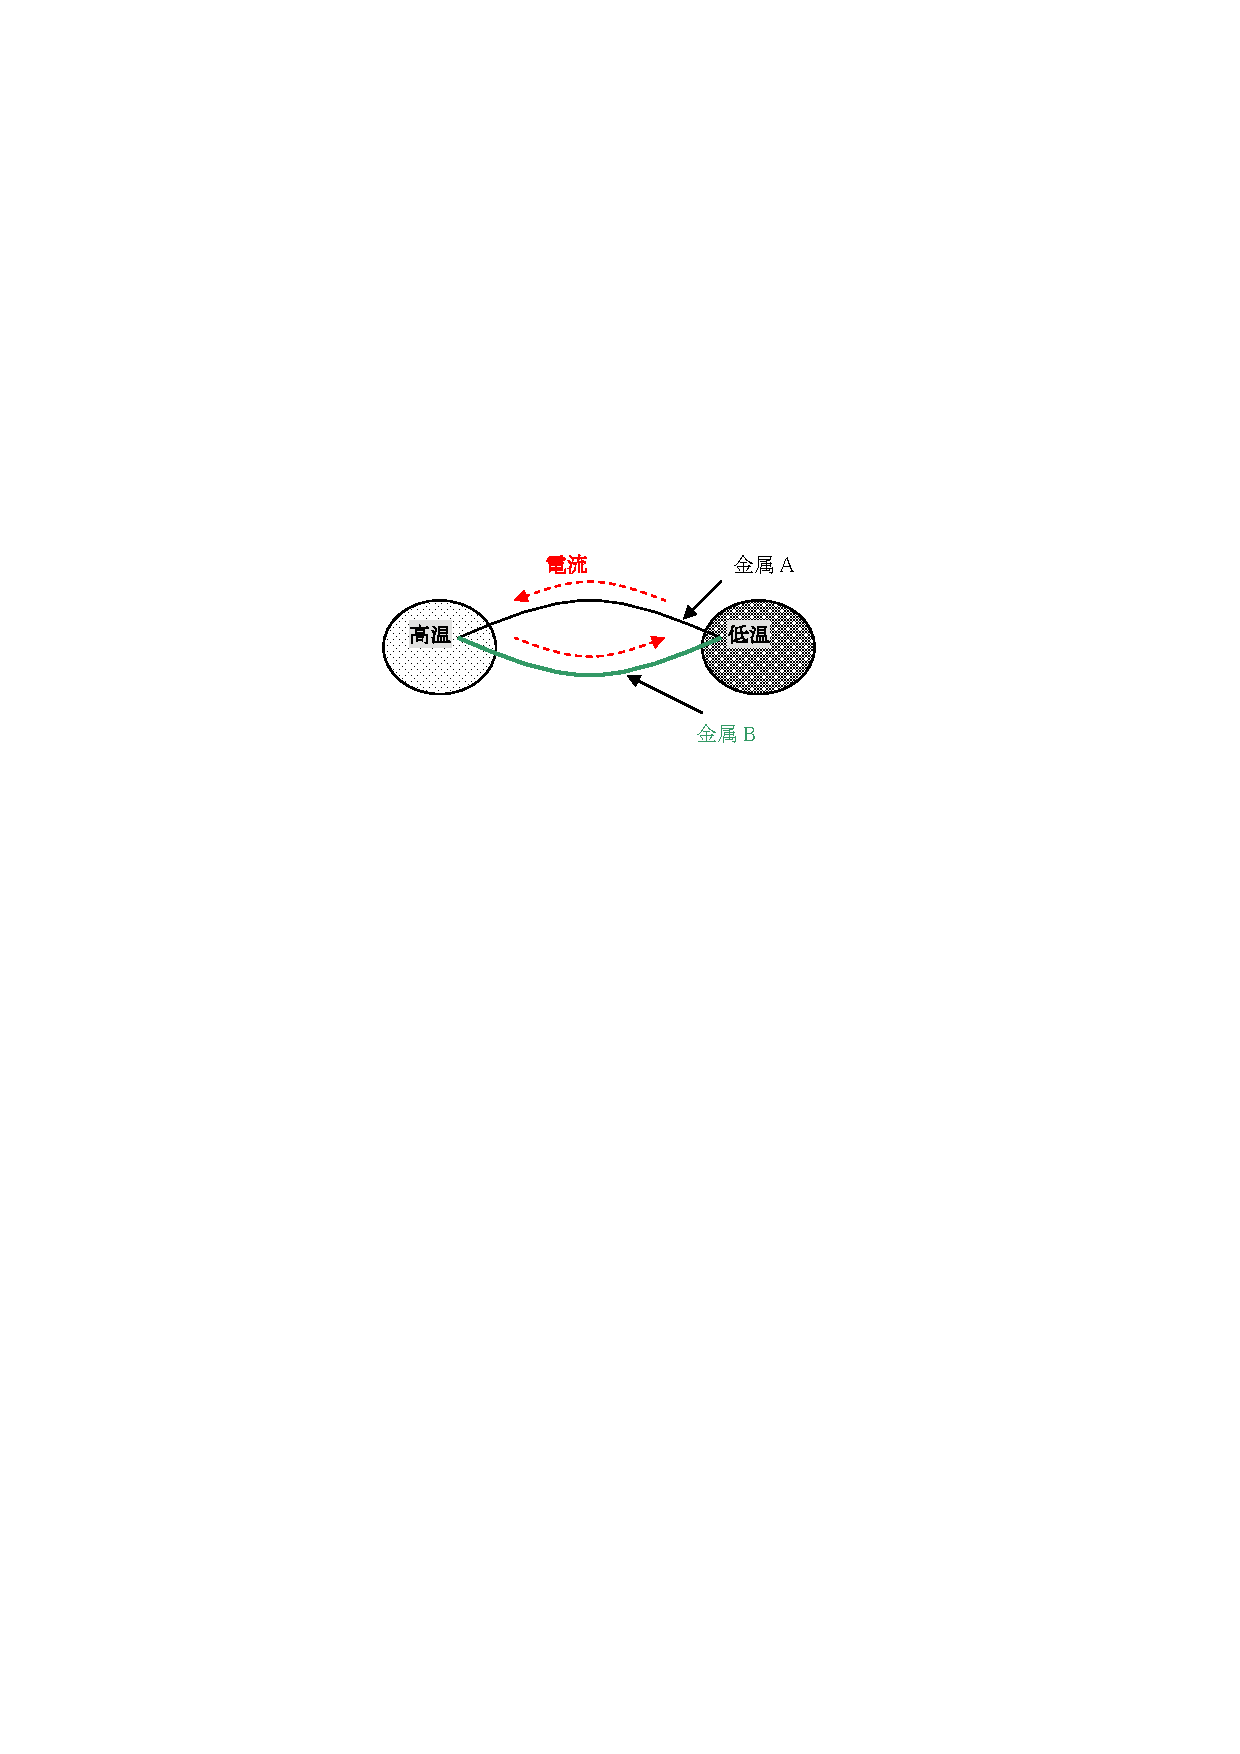
\includegraphics[bb=175 482 441 585]{10_Thermocouple/thermocouple1.pdf}
\end{center}

この熱電対の片方の接点を開いてやれば、下図のようにして、温度差によって生じ 
ている電位差(熱起電力)を測定してやることができます。

\begin{center}
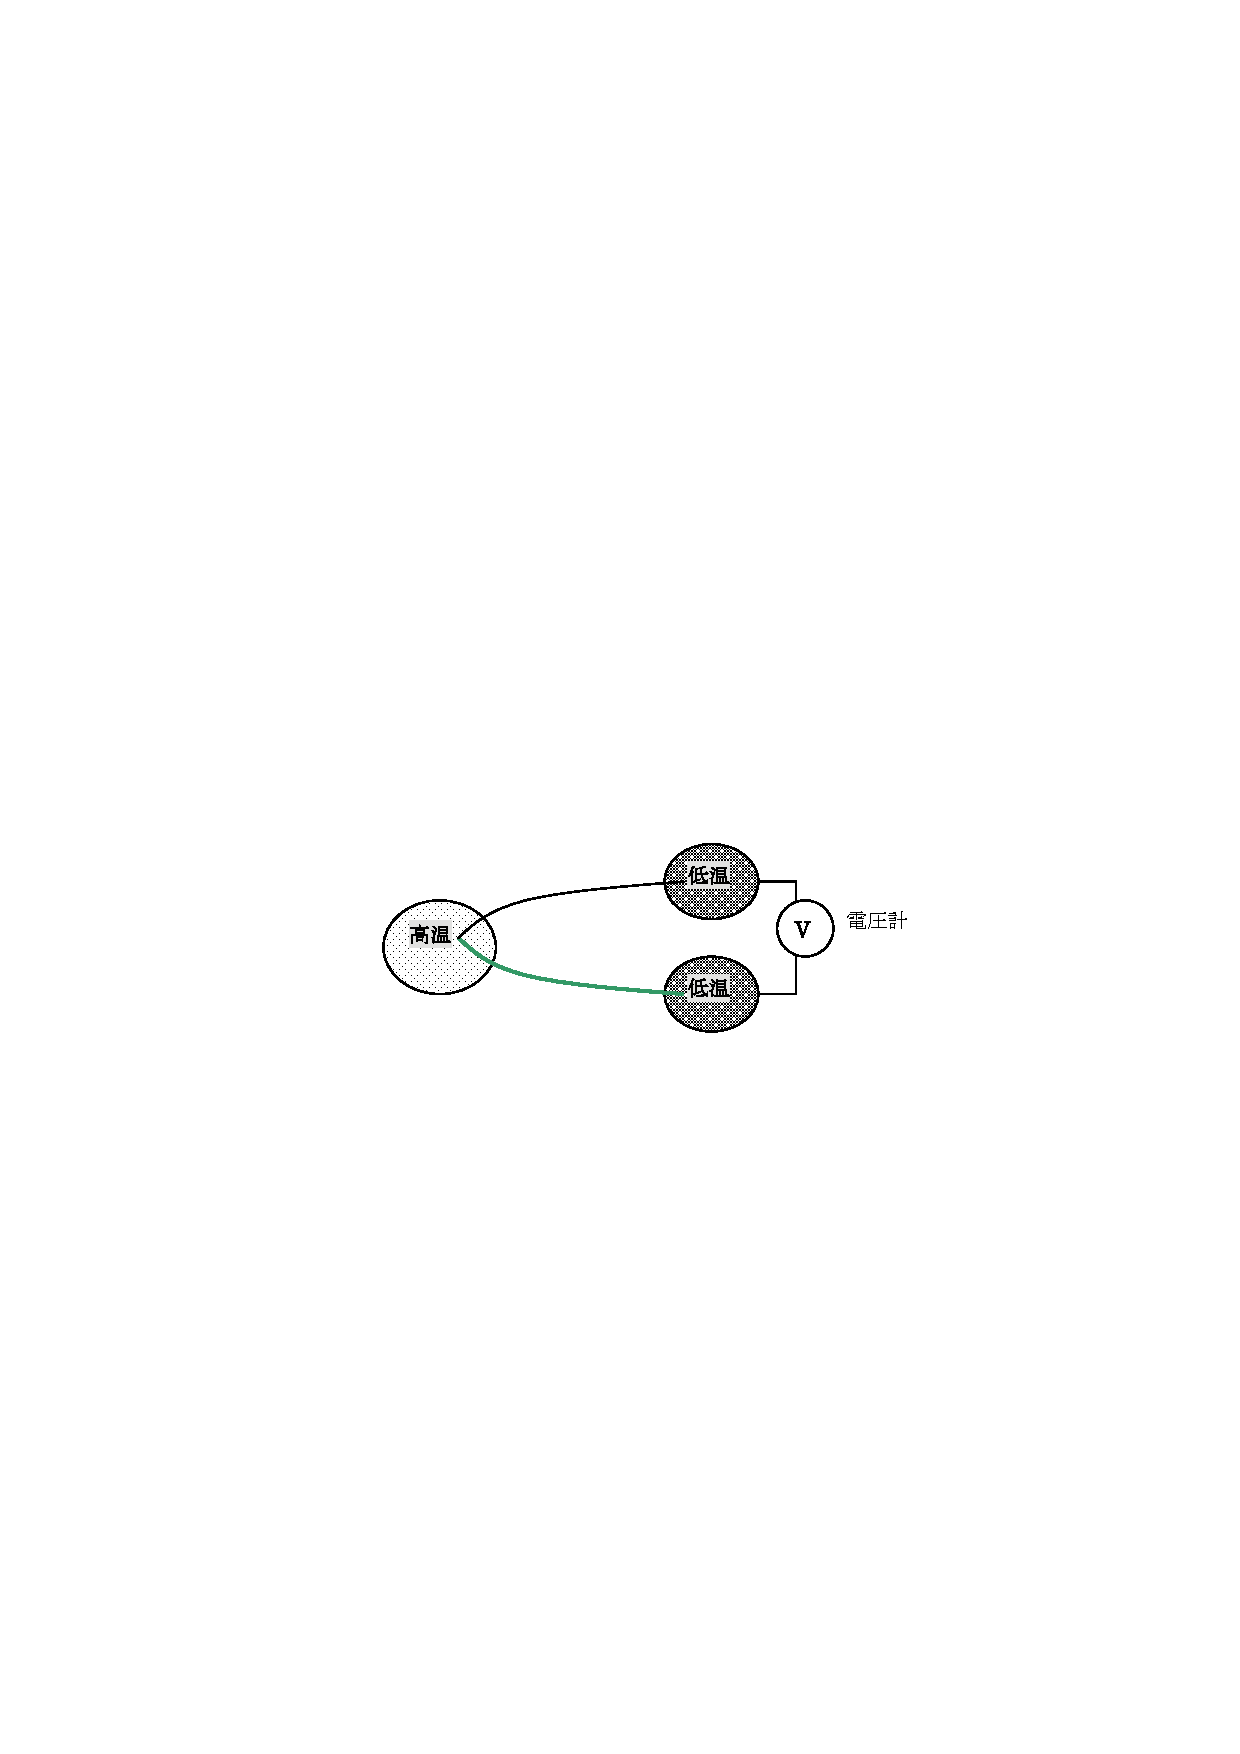
\includegraphics[bb=178 340 443 443]{10_Thermocouple/thermocouple2.pdf}
\end{center}

熱電対の温度差と起電力の関係は組み合わせる金属の種類によって決まり、金属の 
形や大きさには関係しないため、熱起電力が分かっていれば、熱電対を温度の測定に 
使用することができます。測定できる温度の範囲は金属の種類によって異なりますが、 
例えばクロメル−アルメル熱電対では、$-200$℃から1000℃位まで、幅広い温度を測 
定することが可能です。

\subsection{熱起電力が生じる仕組み}

熱電対に生じる熱起電力の原因は、高温接点と低温接点の温度差を無くそうとして 
生じる熱の流れです。熱の流れは金属内の電子が温度の高い部分から低い部分へ向か 
って動くことによって生じますが、電子は電荷を持っているため、電子が動くことに 
よって起電力が生じます。二つの接点の温度差がついたままの状態だと、この起電力 
もそのまま保持されることになります。この原理から予想されるように、接点間の温
度差が大きければ大きいほど、熱の流れ(電子の流れ)も大きくなり、結果として起 
電力は大きくなります。


\subsection{熱起電力の測定}

熱電対を温度計として使用するためには、熱電対の接点の温度差と起電力の関係を 
調べる必要があります。これを実際に実験で求めてみましょう。実験では、クロメル 
-アルメル熱電対を用います。高温接点の温度を変化させ、低温接点との温度差と、 
その時の起電力を測定し、グラフを作成しましょう。

実験で使う熱電対は石英ガラス等で保護してあり、二つに切り開いた低温接点部分 
にそれぞれ補償導線を繋げた形のものです。補償導線には熱電対と同等の熱起電力特 
性を持つものが使用されており、この導線があっても熱起電力の値に大きな影響を与 
えることが無いように工夫されています。

\subsection{ペルティエ素子と熱起電力}

ペルティエ素子はゼーベック効果の逆過程となるペルティエ効果を利用して、電流と共に熱を輸送し温度差を作り出す半導体素子で、CPUやポータブル冷蔵庫の冷却用途として広く使われています。ペルティエ素子は、ゼーベック効果の素子としても機能するため、両面に外部から温度差を与えると、起電力を発生します。ペルティエ素子は多数集積させることで、一対の熱電対よりも高い起電力を発生し、モーターなどの動力も動かすことができます。

放射性同位体の原子核崩壊の際に発生する熱を電気エネルギーに変換するために、ペルティエ素子を用いた熱電発電装置(原子力電池)といったものも開発され、その長い電源寿命を活かして、宇宙探査機等の電源としても利用されています。

\newpage

\jikken

\begin{itemsquarebox}[c]{\bf 実験用具}
恒温水槽、クロメル−アルメル熱電対、接続用ケーブル、スタンド、
温度計、冷接点用接続器(ステンレス製デュワー瓶)、デジタル電圧計、
熱起電力実験器
\end{itemsquarebox}

\bigskip

\subjikken{熱電対の熱起電力の測定}

\begin{enumerate}

\item 冷接点用接続器には氷水を入れ、温度計を挿しておきます。

\item 恒温水槽に高さ5 cm程度まで水を張り、ヒーターをセットします。最初の温度設
定は、水温程度まで下げておきます。

\item クロメル-アルメル熱電対の「クロメル(+)」と書かれた接点と冷接点用接続器の「C」 
と書かれた端子、「アルメル(−)」と書かれた接点と「A」と書かれた端子を、導線で 
それぞれ接続します。接続したら、熱電対の高温接点を恒温水槽の中に入れ、熱 
電対をスタンドなどで固定しておきます。

\item 冷接点用接続器の「C」「A」の下の「+」と「−」と書かれた端子に、導線を使 
ってデジタル電圧計のプローブを接続しておきます。測定は[mV]で行います。

\item 冷接点の温度を記録し、恒温水槽の水温を5℃ずつ上げながら、熱起電力を測定 
していきます(80℃程度まで)。ただし、恒温水槽の温度表示が目的の温度にな 
ってから3分ほど待ち、値が安定した時点で起電力を読み取ること。

\item 恒温水槽から熱電対の高温接点を取り出し、十分に冷ました後に手で握って暖める。値が安定した時点での
起電力を読み取る。

\item 冷接点と高温接点の温度差を横軸、熱起電力を縦軸にとってグラフを作成しましょう。さらに、
このグラフとExcelを用いて、この温度差と熱起電力の関係式を直線で近似した式を求めてみましょ
う。

\item ペルチェ素子を利用した熱起電力実験器を用いて、温度差によって発電ができることを確認しましょう。

\end{enumerate}



